\documentclass[11pt,a4paper]{article}
\usepackage[T1]{fontenc}
\usepackage[utf8]{inputenc}
\usepackage[polish]{babel}
\usepackage{amsmath}
\usepackage{amsfonts}
\usepackage{graphicx}
\author{Kamil Kuczaj}
\title{Sprawozdanie z Laboratorium 6 - Pomiar czasu wyszukiwania klucza w tablicy asocjacyjnej.}
\date{\today}
\begin{document}

\maketitle

\section{Wstęp}
\hspace{4ex}Zadaniem na laboratorium był pomiar czasu wyszukiwania klucza w tablicy asocjacyjnej. Jest ona zbudowana z tablicy asocjacyjnej, która składa się z list niewielkich rozmiarów. Funkcja sortująca przyporządkowuje odpowiedni \textit{bucket} po podaniu do niej klucza (\textit{tj. elementu}. Wg teorii algorytm ten powinien mieć złożoność obliczeniową równą O($1$).\\\\W naszym przypadku mieliśmy załadować kolejno $10^1$, $10^3$, $10^5$, $10^6$, $10^9$ oraz sprawdzić czas wyszukiwania znanego elementu. Konstrukcja tablicy asocjacyjnej przypominała w moim przypadku książkę telefoniczną, tj. na podstawie słowa zwracana była liczba złożona maksymalnie z 9 cyfr.\\\\Na potrzeby zadania został napisany krótki program, który na podstawie zadanego słownika - pobrano angielski składający się z $349900$ wyrażeń - generuje \textit{książkę telefoniczną} przypisując każdemu wyrażeniu losową liczbę całkowitą mniejszą niż $10^10$.\\\\Ponieważ w tablicy asocjacyjnej należało posłużyć się listą, a mój poprzedni kod dla niej wykorzystywał węzły, a nie tablicę posłużyłem się biblioteką \textit{STL} języka \textit{C++} i szablonem \textit{std::list<>}.\\\\Jako \textit{funkcję sortującą} (ang. \textit{hash function}) został obrany algorytm, który oparty był o \textit{Twierdzenie Bézouta}. Istnieje wiele innych, np. \textit{•}\\\\Obsługa kolizji w tablicy asocjacyjnej polega na tym, że nowy element jest po prostu dopisywany. Gdybym uwzględniał ten fakt, nigdy nie mógłbym dodać więcej elementów niż wspomniane $349900$ elementów.\\\\Tablica asocjacyjna zna swój rozmiar od momentu inicjalizacji - nie wystarczyło mi czasu na dodanie tej funkcji. Nie udało mi się również przeprowadzić testów dla miliarda elementów, gdyż zabrakło zasobów fizycznych na komputerze na obsługę takiej listy. Nadmienię iż dla samej tablicy miliarda liczb całkowitych, było wymagane \textbf{5 GB pamięci fizycznej}. Tutaj dochodzi do tego zmienna typu std::string, która zajmuje dwa razy więcej pamięci. Dlatego, aby wykonać test dla miliarda elementów tego typu, komputer potrzebuje co najmniej \textbf{15 GB pamięci podręcznej}. W przeciwnym wypadku korzystając z pliku stronicowania, którego szybkość odczytu zależy od zastosowanego typu dysku twardego, proces ten będzie trwał bardzo długo.

\section{Specyfikacja komputera}

\begin{center}
	\begin{tabular}{| r | c |}
	\hline
	Wersja kompilatora \textit{g++} & 4.8.4 \\ \hline
	System & Ubuntu 14.04.4 \\ \hline
	Procesor	 & Intel Core i5 2510M 2.3 GHz \\ \hline
	Pamięć RAM & 8 GB DDR3 1600 MHz \\ \hline
	Dysk twardy & HDD (5400 obr./min) \\ \hline
	Rozmiar zmiennej \textit{int} & 4 bajty \\ \hline
	Rozmiar zmiennej \textit{std::string} & 8 bajty \\ \hline	
	\end{tabular}
\end{center}

\section{Pomiary oraz ich interpretacja}

\begin{table}[htbp]
\caption{}
\begin{center}
\begin{tabular}{|r|r|r|r|}
\hline
\multicolumn{ 4}{|c|}{\textbf{Tablica hashowa – wyniki w mikrosekundach $\mu s$}} \\ \hline
\textbf{10} & \textbf{1000} & \textbf{100000} & \textbf{1000000} \\ \hline
30 & 8 & 24 & 30 \\ \hline
5 & 14 & 27 & 38 \\ \hline
4 & 26 & 25 & 32 \\ \hline
4 & 18 & 26 & 30 \\ \hline
3 & 19 & 26 & 28 \\ \hline
4 & 19 & 27 & 27 \\ \hline
4 & 21 & 27 & 29 \\ \hline
4 & 22 & 28 & 27 \\ \hline
4 & 21 & 27 & 26 \\ \hline
4 & 17 & 26 & 31 \\ \hline
4 & 16 & 35 & 31 \\ \hline
4 & 17 & 31 & 26 \\ \hline
3 & 22 & 28 & 26 \\ \hline
3 & 15 & 26 & 29 \\ \hline
\end{tabular}
\end{center}
\label{Wyniki pomiarów1}
\end{table}


\begin{table}[htbp]
\caption{}
\begin{center}
\begin{tabular}{|r|r|r|r|}
\hline
\multicolumn{ 4}{|c|}{\textbf{Tablica hashowa – wyniki w mikrosekundach $\mu s$}} \\ \hline
\textbf{10} & \textbf{1000} & \textbf{100000} & \textbf{1000000} \\ \hline
4 & 15 & 36 & 29 \\ \hline
4 & 17 & 27 & 35 \\ \hline
4 & 16 & 27 & 38 \\ \hline
4 & 19 & 38 & 40 \\ \hline
4 & 14 & 27 & 41 \\ \hline
3 & 14 & 26 & 28 \\ \hline
4 & 19 & 26 & 27 \\ \hline
4 & 18 & 36 & 28 \\ \hline
4 & 15 & 31 & 28 \\ \hline
3 & 14 & 26 & 28 \\ \hline
4 & 13 & 26 & 28 \\ \hline
4 & 14 & 31 & 31 \\ \hline
4 & 14 & 28 & 27 \\ \hline
4 & 59 & 26 & 26 \\ \hline
4 & 14 & 27 & 27 \\ \hline
4 & 14 & 26 & 27 \\ \hline
3 & 14 & 25 & 36 \\ \hline
3 & 13 & 25 & 27 \\ \hline
4 & 12 & 26 & 28 \\ \hline
4 & 13 & 27 & 30 \\ \hline
4 & 12 & 26 & 28 \\ \hline
3 & 13 & 28 & 32 \\ \hline
4 & 13 & 27 & 28 \\ \hline
3 & 13 & 27 & 37 \\ \hline
4 & 12 & 31 & 28 \\ \hline
4 & 12 & 35 & 28 \\ \hline
3 & 13 & 27 & 26 \\ \hline
4 & 13 & 28 & 28 \\ \hline
4 & 12 & 25 & 28 \\ \hline
4 & 13 & 27 & 37 \\ \hline
3 & 13 & 39 & 30 \\ \hline
4 & 21 & 34 & 29 \\ \hline
4 & 13 & 25 & 27 \\ \hline
3 & 13 & 27 & 26 \\ \hline
4 & 25 & 28 & 27 \\ \hline
4 & 28 & 27 & 28 \\ \hline
\multicolumn{1}{|l|}{} & \multicolumn{1}{l|}{} & \multicolumn{1}{l|}{} & \multicolumn{1}{l|}{} \\ \hline
\multicolumn{ 4}{|c|}{\textbf{Średnie czasów [$\mu s$]}} \\ \hline
4,3 & 16,7 & 28,22 & 29,72 \\ \hline
\end{tabular}
\end{center}
\label{Wyniki pomiarów2}
\end{table}


\begin{figure}[htbp]
\begin{center}
	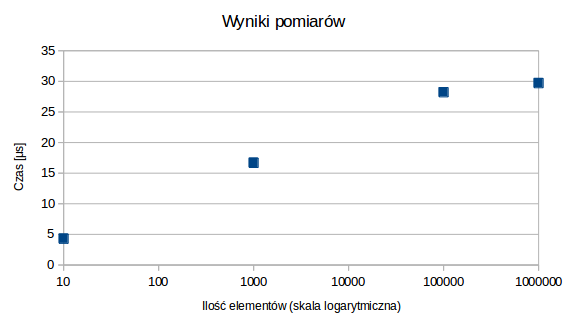
\includegraphics[scale=0.7]{wykres.png}
\end{center}
\end{figure}


\section{Wnioski}
\hspace{4ex}Wyraźnie widać po wynikach pomiarów, że dostęp do każdego elementu jest błyskawiczny. Widać jednak, że w skali logarytmicznej punkty układają się mniej więcej na linii prostej, co implikuje to, że złożonośc obliczeniowa w czasie mojej listy asocjacyjnej to O($log(n)$), a nie O($1$), tak jak mówi teoria. Być może odpowiedzialny jest za to algorytm haszujący.
\end{document}